\documentclass[12pt,a4paper]{article}
\usepackage[utf8]{inputenc}
\usepackage{graphicx}
\usepackage{float}
\usepackage{subcaption}
\usepackage[margin=1in]{geometry}
\usepackage{hyperref}  
\hypersetup{
  pdfborder = {0 0 0}
}
\usepackage[
backend=biber,
style=alphabetic,
]{biblatex}

\addbibresource{radio.bib}

\graphicspath{{./Pictures/}}
\DeclareGraphicsExtensions{.pdf,.jpeg,.jpg,.png}

\usepackage{amsmath} % equations
\usepackage{fancyhdr} % nicer page header
\usepackage{listings} % For inclusion of code



\setlength{\parindent}{0pt} % no paragraph indents
\setlength{\parskip}{1em} % paragraphs separated by one line

\newcommand\experiment{Experiment Radio astronomy} %%%%% experiment name
\newcommand\groupno{Group 3+12}       %%%%% group number
\newcommand\names{Pratyush Singh,\\
                  Proshmit Dasputpa,\\
                  Dhruv Nahar}        %%%%% full names
\newcommand\expdate{25/03/2025}    %%%%% date of experiment day

\begin{document}
\begin{titlepage}
   \begin{center}
        \vspace*{3cm}
        \Huge{\experiment}
				
        \vspace{0.5cm}
        \LARGE{Lab course protocol}
				
        \vspace{3 cm}
        \Large{\groupno}
				
        \vspace{0.25cm}
        \large{\names}
				
        \vspace{2 cm}
        \Large{\expdate}
				
        \vspace{0.25 cm}
        \Large{Advanced lab course in astronomy\\
				Eberhard Karls Universit\"at T\"ubingen}
				
				\vspace{0.1 cm}
        \Large{WiSe 2024/25}
				
       \vfill
    \end{center}
\end{titlepage}

\pagestyle{fancy}
\fancyhf{}
\setlength{\headheight}{14.5pt}
\lhead{\groupno; \experiment}

% \section*{Abstract}
% This is optional, but never longer than half a page.

\tableofcontents
\newpage

\setcounter{page}{1}
\pagestyle{fancy}
\fancyhf{}
\rhead{\thepage}
\lhead{\groupno; \experiment}

\section{Introduction}\label{sec:intro} % labels allow references, particularly important for figures and tables

In this experiment, we explore the fundamentals of radio astronomy using the Tübingen Radio Telescope located at Sand $1$. Unlike optical astronomy (limited by interstellar dust), radio observations provide a powerful tool to study regions of the galaxy otherwise obscured. This lab focuses on two key radio sources: the Sun and the Milky Way. 

Radio astronomy began with Karl Jansky's discovery of extraterrestrial radio waves in the 1930s, marking the birth of a new observational window in astrophysics. Since then, radio observations have led to significant breakthroughs, including the discovery of pulsars, the cosmic microwave background, and compelling evidence for dark matter.

During this lab, we detect thermal radio emission from the Sun and the 21 cm hyperfine line of neutral hydrogen (H\,\textsc{i}) in the Milky Way. The experiment involves measuring Doppler shifts in the 21 cm line to derive the galaxy's rotation curve and estimate the distribution of interstellar gas. Observations will be conducted with a 2.3-meter radio telescope, with the aim of gaining practical experience in data acquisition, calibration, and analysis.

The goals are to understand the operation of a radio telescope, explore the rotation dynamics of our galaxy, and practice converting observational data into astrophysical insights such as the mass distribution within the Milky Way.

\paragraph{\textbf{Origin and type of radiation emitted by the galactic center:}}
The galactic center emits non-thermal radio radiation, primarily in the form of \textit{synchrotron radiation}. This type of emission is produced by relativistic electrons spiraling around magnetic field lines. The source of this radiation is the region surrounding the supermassive black hole at the center of the Milky Way, known as \textbf{Sagittarius A*}, which is a strong and compact radio source.

\section{Theory}
\label{sec:theory}
  \subsection{The Sun}
  The Sun is the brightest discrete radio source in the sky and serves as a primary target in radio astronomy experiments, particularly with small telescopes. In this experiment, the Sun is observed as a point source, since the telescope's angular resolution is not sufficient to resolve its disk.

The angular resolution $\theta$ of a radio telescope is given approximately by the diffraction formula:
\[
\theta \approx \frac{\lambda}{D}
\]
where $\lambda \sim 21\,\mathrm{cm}$ is the observed wavelength and $D = 2.3\,\mathrm{m}$ is the diameter of the telescope's dish. This yields an angular resolution of about $5^\circ$, significantly larger than the angular diameter of the Sun (approximately $0.5^\circ$). Thus, the Sun appears as an unresolved source, and its exact position and the beam width of the telescope can be determined by scanning across its location.

Unlike optical emission, which originates from the photosphere, the radio emission from the Sun primarily comes from its chromosphere and corona. This emission is of thermal origin and varies with solar activity, particularly in active regions associated with sunspots and magnetic phenomena.

In the experiment, we may perform a raster scan across the Sun's position using the equatorial coordinate system. By scanning across Right Ascension (RA) and Declination (DEC) independently and measuring the radio intensity, the beam profile of the telescope can be reconstructed. The peak of the intensity corresponds to the Sun's position, and the beam width can be estimated from the full width at half maximum (FWHM) of the Gaussian fit to the intensity profile. 

A linear scan may also be performed, where only one coordinate (RA or DEC) is varied while the other is kept constant. This method is less time-consuming and can be used to measure the beam width in one dimension. The intensity profile is then fitted with a Gaussian function to determine the FWHM.

\paragraph{\textbf{Preferred coordinate system and scan parameters:}}
For this part of our experiment, the \textit{equatorial coorrdinate system} is preferred, as it remains fixed relative to the celestial sphere. The equatorial coordinates (RA and DEC) remain essentially constant for short observation periods. This makes it easier to conduct scans - especially when tracking or mapping point sources like the Sun. Moreover, these coordinates align \\ naturally with astronomical catalogs - simplifying telescope control.

The angular resolution (beam width) of the telescope is approximately \( 5^\circ \). To capture the full intensity profile of the Sun, the scan should extend over a range of \( \pm 10^\circ \). A step size of \( 2^\circ \) provides a good resolution for the scan. Therefore, the total number of measurement points is:

\[
\text{Number of points} = \frac{20^\circ}{2^\circ} + 1 = 11
\]
\\ Meanwhile, the right ascension is measured in time units, where:

\[
360^\circ = 24\ \text{hours} \Rightarrow 1^\circ = 4\ \text{minutes}
\]

Thus, a step size of \( 2^\circ \) corresponds to: 
\[
\boxed{
2^\circ = 8\ \text{minutes} = 0^\text{h}08^\text{m}00^\text{s}
}
\]

\noindent So the scan should proceed in steps of \( 2^\circ \) in declination or \( 0^\text{h}08^\text{m}00^\text{s} \) in right ascension.

This part of the experiment introduces key observational techniques in radio astronomy with the aim of providing a direct measurement of the telescope’s spatial resolution.

  \subsection{Doppler Effect}


  The Doppler effect describes the change in frequency (or wavelength) of a wave due to the relative motion between the source and the observer. This effect has been named after the Austrian physicist Christian Johann Doppler (1803-1853). In the context of radio astronomy, it is crucial for measuring the radial velocity of gas clouds in the Milky Way via their emission lines, particularly the 21 cm line of neutral hydrogen.
  
  Assuming a source moving with velocity $v$ along the line of sight (toward or away from the observer), the observed frequency $f$ is shifted relative to the emitted frequency $f_0$:
  \[
  \frac{\Delta f}{f_0} = \frac{f - f_0}{f_0} = -\frac{v}{c}
  \]
  where $c$ is the speed of light. A negative $\Delta f$ (i.e., $f < f_0$) corresponds to a redshift (source moving away), while a positive $\Delta f$ indicates a blueshift (source approaching).
  
  In wavelength terms, the corresponding relation is:
  \[
  \frac{\Delta \lambda}{\lambda_0} = \frac{v}{c}
  \]
  valid for non-relativistic velocities ($v \ll c$). The small frequency shifts caused by gas motions in the Milky Way are detectable using sensitive radio receivers tuned around the rest frequency of the 21 cm line ($f_0 = 1420\,\mathrm{MHz}$).
  

\paragraph{Derivation from the wavelength to frequency relation:}

We start from the \\ expression for the Doppler effect in terms of wavelength:

\begin{equation}
\frac{\Delta \lambda}{\lambda_0} = \frac{v}{c} \tag{2.1}
\end{equation}

The frequency \( f \) and wavelength \( \lambda \) are related by:

\[
f = \frac{c}{\lambda}
\quad \Rightarrow \quad
\lambda = \frac{c}{f}
\]

Taking a differential of \( f = \frac{c}{\lambda} \) gives:

\[
\Delta f = \frac{d}{d\lambda}\left(\frac{c}{\lambda}\right) \cdot \Delta \lambda 
= -\frac{c}{\lambda^2} \cdot \Delta \lambda
\]

Now dividing both sides by \( f = \frac{c}{\lambda} \) to obtain the relative change:

\[
\frac{\Delta f}{f} = -\frac{\Delta \lambda}{\lambda}
\]

Substituting equation (2.1) into this expression:

\[
\frac{\Delta f}{f} = -\frac{v}{c}
\]

\begin{equation}
\boxed{
\frac{\Delta f}{f} = -\frac{v}{c}
}
\tag{2.2}
\end{equation}

This is the Doppler shift in terms of frequency (exercise solved).

By measuring the frequency shift $\Delta f$ of the hydrogen line, we can infer the radial velocity $v_r$ of the emitting gas along our line of sight. These measurements are fundamental to constructing the galaxy’s rotation curve and studying its mass distribution.
  
  In the experiment, spectra of the Milky Way are recorded at various galactic longitudes, and the velocities of the hydrogen gas clouds are extracted from the Doppler-shifted emission lines using this principle.
   

  \subsection{The Milky Way}

The Milky Way is our home galaxy, composed of stars, gas, dust, and dark matter arranged in a spiral structure. From Earth, it appears as a bright band across the sky. Observations from within are complicated by interstellar dust, which blurs many regions in the optical band. However, radio waves — particularly the 21\,cm line of neutral hydrogen — can penetrate this dust, allowing us to study the galaxy's structure and dynamics.

To describe positions in the sky, several coordinate systems are used. For galactic studies, the \textit{galactic coordinate system} is most convenient, where longitude \( l \) measures angular distance from the galactic center and latitude \( b \) indicates vertical distance from the galactic plane.
\begin{figure}[H]
  \centering
  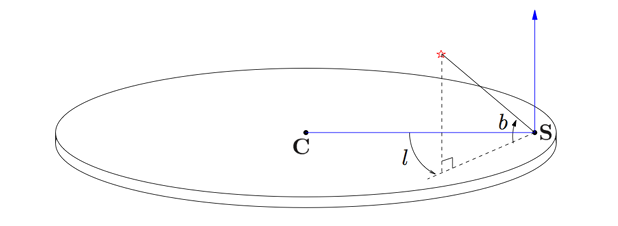
\includegraphics[width=0.6\textwidth]{Pictures/bl.png}
  \caption{Galactic coordinates \( l \) and \( b \) in the Milky Way.}
  \label{fig:bl}
\end{figure}
\paragraph{Reason why the two coordinates \( l \) and \( b \) are sufficient to describe the (three-dimensional) Milky Way, and addressing whether this is always the case:} 
The galactic coordinates \( l \) (longitude) and \( b \) (latitude) define the direction to an object on the sky, sufficient for a two-dimensional angular map of the Milky Way. To obtain three-dimensional data, the distance along the line of sight is needed. In radio astronomy, this is often inferred from Doppler-shifted velocities and an assumed galactic rotation model. However, this approach introduces ambiguities and assumptions, and is not always reliable. This is true especially in directions where multiple distances correspond to the same radial velocity, or in regions with non-circular gas motions.

Observing neutral hydrogen in these coordinates helps to map the spiral arms and motion of gas in the disk of the galaxy. Neutral hydrogen (H\,\textsc{i}) is the most abundant element in the interstellar medium and can be detected via its characteristic 21\,cm hyperfine line, corresponding to a frequency of 1420\,MHz. This line arises from a spin-flip transition in the hydrogen atom and, despite its low probability, is prominent due to the vast quantity of hydrogen in the galaxy.
\begin{figure}[H]
  \centering
  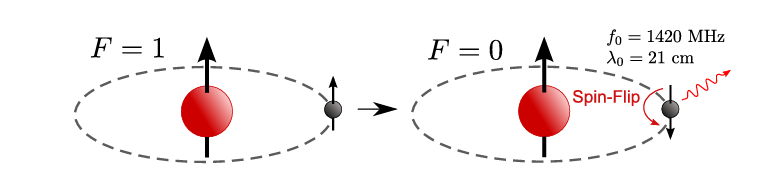
\includegraphics[width=1.0\textwidth]{Pictures/hydrogen.png}
  \caption{Hyperfine structure transition of neutral hydrogen. (Credit: \cite{enwiki:1280656493})}
  \label{fig:spin}
\end{figure}
\paragraph{\textbf{Addressing the exercise:}}
The 21\,cm line can be easily observed because:
\begin{itemize}
    \item It lies in the radio part of the spectrum, which penetrates interstellar dust and allows observations throughout the entire Galaxy.
    \item Hydrogen is the most abundant element, ensuring widespread and strong emission.
    \item The narrow line allows precise measurement of Doppler shifts, giving velocity information about the gas.
\end{itemize}

Other tracers used for similar purposes include:
\begin{itemize}
    \item \textbf{CO (Carbon Monoxide)} – Traces molecular hydrogen (H$_2$) in star-forming regions. (\cite{bolatto2013co})
    \item \textbf{H$\alpha$ emission} – Traces ionized hydrogen in regions with active star formation, though it is subject to dust extinction. (\cite{kennicutt1998star})
    \item \textbf{Infrared emission} – Traces warm dust and embedded star-forming regions. (\cite{belfiore2023calibrating})
\end{itemize}
Thus by observing the 21\,cm emission, we can trace the distribution and velocity of hydrogen gas clouds. These observations are fundamental for constructing a map of the Milky Way and understanding its rotation. The Doppler shift of the line provides velocity information, which is critical for determining the motion of gas and estimating the galaxy’s mass distribution.



\subsubsection*{Geometry}

\begin{figure}[H]
  \centering
  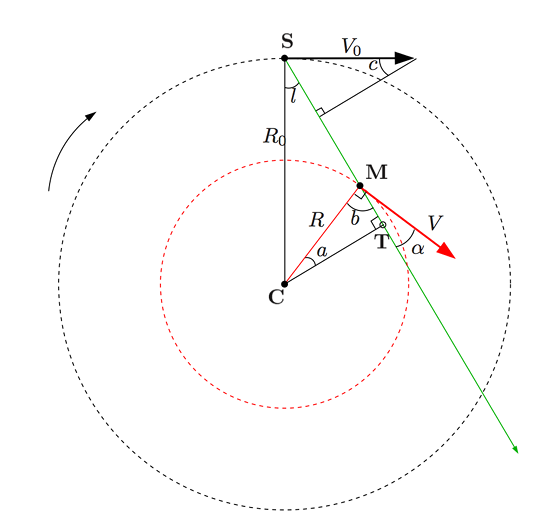
\includegraphics[width=0.6\textwidth]{Pictures/geometry.png}
  \caption{Geometry of the Milky Way}
  \label{fig:geometry}
\end{figure}

To analyze the motion of hydrogen gas within the Milky Way, we consider the geometry of the Galaxy in galactic coordinates. Observations are made from the Sun's position, which lies at a distance $R_0 = 8.5\,\mathrm{kpc}$ from the galactic center. The gas clouds in the galaxy orbit the center, and their velocity vectors form an angle with our line of sight. 

The observed radial velocity $V_r$ (or line-of-sight velocity) is the projection of a cloud's true orbital velocity $V$ onto the observer's line of sight, corrected for the Sun's own motion. This can be expressed as:
\[
V_r = V \cos \alpha - V_0 \sin l
\]
where:
\begin{itemize}
  \item $V$ is the orbital velocity of the gas cloud,
  \item $V_0$ is the Sun's orbital velocity around the galactic center ($\sim220\,\mathrm{km/s}$),
  \item $l$ is the galactic longitude of the line of sight,
  \item $\alpha$ is the angle between the cloud's velocity vector and the line of sight.
\end{itemize}

Using trigonometry and assuming circular orbits, it can be shown that:
\[
\cos \alpha = \frac{R_0 \sin l}{R}
\]
Substituting this into the expression for $V_r$, we obtain:
\[
V_r = V \cdot \frac{R_0 \sin l}{R} - V_0 \sin l
\]

This relationship allows us to derive important kinematic properties of the galaxy from observed spectral line shifts. It is especially useful when applied to the tangent point method (described in the next section), where the projection geometry simplifies \\ significantly.

  
    \subsubsection*{Milky Way Rotation}

The rotation of the Milky Way can be studied by analyzing how the orbital velocity of gas varies with distance from the Galactic center. This relationship is known as the \emph{rotation curve}. There are three forms of rotation:

\begin{itemize}
  \item \textbf{Solid-body rotation:} All parts of the system rotate with the same angular \\ velocity $\Omega$, so the linear velocity increases linearly with radius:
  \[
  V(R) = \Omega R
  \]
  
  \item \textbf{Keplerian rotation:} For systems dominated by a central mass (e.g., the Solar System), the gravitational acceleration provides the centripetal force:
  \[
  \frac{V^2}{R} = \frac{GM}{R^2} \quad \Rightarrow \quad V(R) = \sqrt{\frac{GM}{R}}
  \]
  This implies that velocity decreases with increasing radius.

  \item \textbf{Differential rotation (flat rotation curve):} In galaxies like the Milky Way, mass is not concentrated at the center but is distributed throughout the disk. Observations show that beyond a certain radius, the orbital velocity remains nearly constant:
  \[
  V(R) \approx \text{const}
  \]
  This implies that the mass continues to increase with radius, even where there is little visible matter — therefore providing evidence for dark matter.
\end{itemize}
\begin{figure}[H]
  \centering
  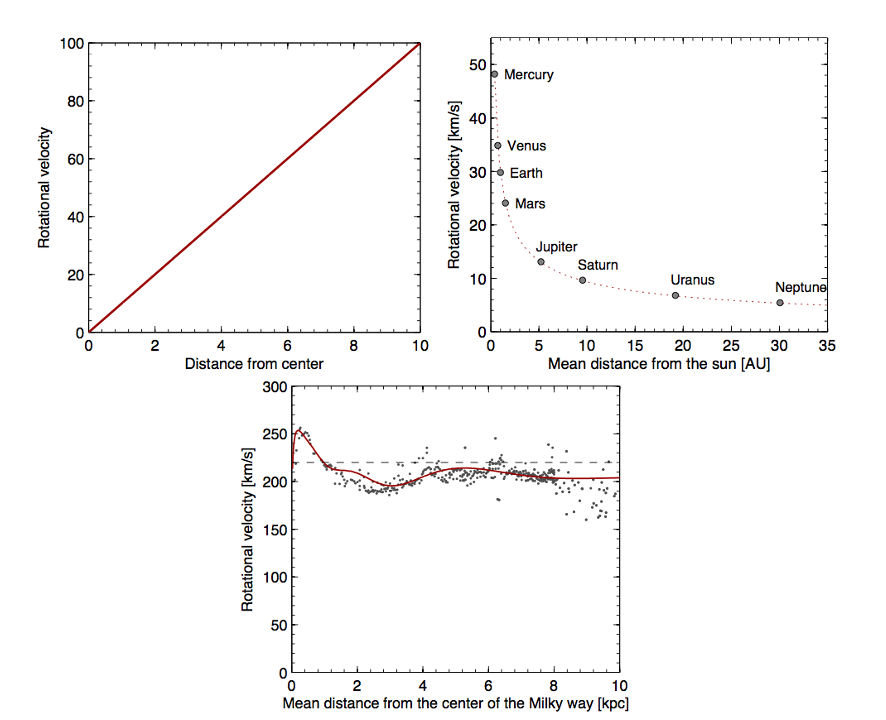
\includegraphics[width=0.8\textwidth]{Pictures/rotation.png}
  \caption{Rotational curves for three types of rotation (clockwise): Solid-body, Keplerian and Differential}
  \label{fig:rotation}
\end{figure}
To measure the rotation curve, we use the \emph{tangent point method} in the inner Galaxy ($0^\circ < l < 90^\circ$). At the tangent point, the velocity vector of a gas cloud is aligned with the line of sight, maximizing the observed radial velocity. The radius of the tangent point is:
\[
R = R_0 \sin l
\]
and the orbital velocity at that point can be calculated as:
\[
V(R) = V_{r,\text{max}} + V_0 \sin l
\]
where $V_{r,\text{max}}$ is the maximum radial velocity observed at longitude $l$.
\paragraph{Applicability of the Tangent Point Method:}
This method is applicable only in the first and fourth galactic quadrants:
\[
0^\circ < l < 90^\circ \quad \text{and} \quad 270^\circ < l < 360^\circ
\]
In these regions, the observer’s line of sight from the Sun passes through the inner part of the galaxy, where it becomes tangent to the circular orbit of the gas at a single point — the \emph{tangent point}.

In contrast, for galactic longitudes \(90^\circ < l < 270^\circ\), the line of sight does not pass through any tangent point within the solar orbit, making the method invalid in these quadrants.

By repeating this for different values of $l$, we can reconstruct the rotation curve $V(R)$ of the Milky Way.

\subsubsection*{Location of the Gas}

In addition to measuring radial velocities, we aim to determine the spatial distribution of neutral hydrogen (H\,\textsc{i}) gas within the Milky Way. Once the Galaxy’s rotation curve $V(R)$ is known, the position of a gas cloud along a line of sight can be inferred from its observed radial velocity.

Assuming circular rotation and using the Doppler formula, the radial velocity is:
\[
V_r = V(R) \cos \alpha - V_0 \sin l
\]
which, using $\cos \alpha = \frac{R_0 \sin l}{R}$ and assuming $V(R) \approx V_0$, simplifies to:
\[
V_r = V_0 \sin l \left( \frac{R_0}{R} - 1 \right)
\]
Solving for $R$ gives:
\[
R = \frac{R_0 V_0 \sin l}{V_0 \sin l + V_r}
\]

Once the Galactocentric distance $R$ is determined, the distance $r$ from the Sun can be found using the law of cosines:
\[
R^2 = R_0^2 + r^2 - 2R_0 r \cos l
\]
Solving this quadratic equation gives two possible solutions for $r$:
\[
r_{\pm} = R_0 \cos l \pm \sqrt{R^2 - R_0^2 \sin^2 l}
\]

\paragraph{Ambiguity of Solutions:}
In the first and fourth Galactic quadrants ($0^\circ < l < 90^\circ$ and $270^\circ < l < 360^\circ$), two positive solutions exist, leading to ambiguity in the cloud's true distance. In contrast, in the second and third quadrants ($90^\circ < l < 270^\circ$), only one solution is physically valid. Additional information, such as vertical position $b$ or assumptions about galactic structure, can help resolve this ambiguity.

Besides determining the rotation curve of the Milky Way, the 21\,cm line measurements allow us to extract additional valuable information about the structure and composition of the galaxy. In particular, we can:

\begin{enumerate}
    \item \textbf{Map the Spiral Structure of the Galaxy:} \\
    Knowing the galactic longitude $l$ and the distance $r$, the position of each gas cloud can be converted to Cartesian coordinates in the Galactic plane:
\[
x = r \cos(l - 90^\circ), \quad y = r \sin(l - 90^\circ)
\]
where the origin is placed at the Sun’s position. A collection of such points allows the construction of a map of the Milky Way’s spiral structure.

This technique reveals large-scale features such as spiral arms, gas rings, and voids, providing insights into Galactic dynamics and evolution.
\begin{figure}[H]
  \centering
  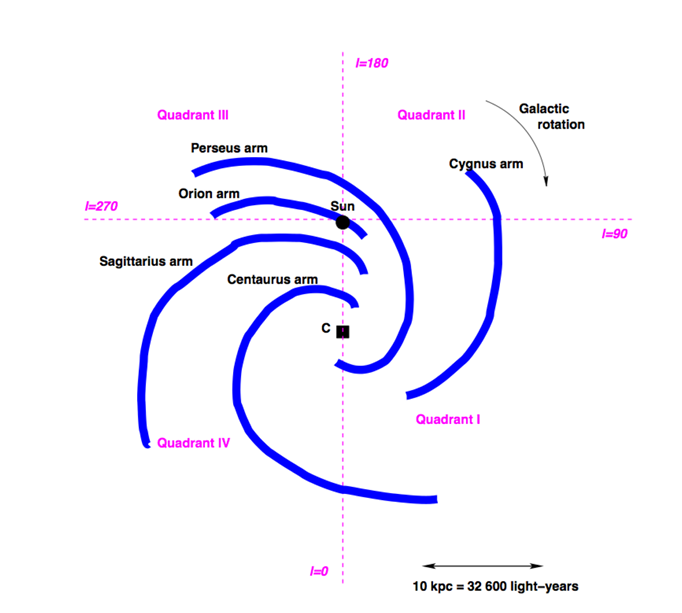
\includegraphics[width=0.7\textwidth]{Pictures/spiral.png}
  \caption{Schematic representation of the Milky Way's spiral structure.}
  \label{fig:spiral}
\end{figure}
    \item \textbf{Detect anomalies (like dark matter distribution):} \\
    If rotation speeds remain constant at large radii instead of decreasing (Keplerian decline), it implies the presence of dark matter.
    
    \item \textbf{Identify Star-Forming Regions:} \\
    Regions of strong H\,\textsc{i} emission, particularly those coinciding with molecular gas (e.g., CO observations), often indicate areas of active or recent star formation (\cite{starform}). These may be associated with giant molecular clouds or H\,\textsc{ii} regions.

\end{enumerate}

\paragraph{Summary of Steps:}
\begin{itemize}
    \item $V_r$ is measured for each observed position $l$.
    \item The rotation curve is used to calculate $R$.
    \item Then one needs to solve for distance $r$ using the law of cosines.
    \item These distances are converted to $(x, y)$ coordinates in the Galactic plane.
    \item Spatial distribution and intensity patterns are analysed.
\end{itemize}

These steps provide a two-dimensional map of the Milky Way's neutral hydrogen and reveal large-scale galactic structure beyond what can be inferred from kinematics alone.
\begin{figure}[H]
  \centering
  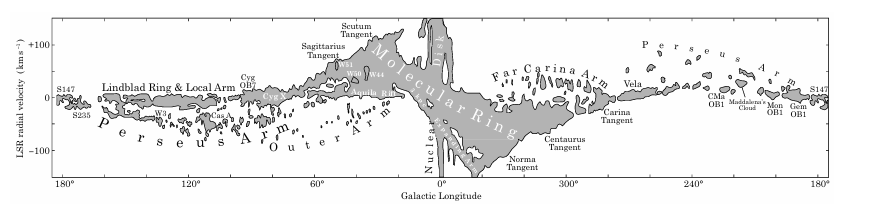
\includegraphics[width=1.0\textwidth]{Pictures/map.png}
  \caption{Portrait of the Milky Way in $v - l$ space. (Credit: \cite{MWMC})}
  \label{fig:map}
\end{figure} 


    \subsubsection*{Mass Estimate of our Galaxy}

The rotation curve of the Milky Way provides a way to estimate the total mass enclosed within a given galactocentric radius. If we assume the galaxy’s mass is spherically \\ distributed (a valid approximation at large radii where the dark matter halo dominates), we can use Newtonian dynamics to calculate the mass. \\ This assumption is in accordance with Jeans theorem - which states that if the mass distribution is spherically symmetric, the motion of matter at a radius R is the same as if all the mass is concentrated in one central point.

The gravitational force provides the necessary centripetal acceleration for circular orbits:
\[
\frac{V^2}{R} = \frac{GM(<R)}{R^2}
\]
Solving for the enclosed mass $M(<R)$ gives:
\[
M(<R) = \frac{V^2 R}{G}
\]
where:
\begin{itemize}
  \item $V$ is the orbital velocity at radius $R$,
  \item $G$ is the gravitational constant ($G \approx 6.674 \times 10^{-11}\,\mathrm{m^3\,kg^{-1}\,s^{-2}}$).
\end{itemize}

In practice, this formula allows us to estimate the mass within the orbit of the Sun, taking:
\[
V \approx 220\,\mathrm{km/s}, \quad R_0 = 8.5\,\mathrm{kpc}
\]
First, $R_0$ is converted to meters from kiloparsecs:
\[
R_0 = 8.5\,\mathrm{kpc} = 8.5 \times 3.086 \times 10^{19}\,\mathrm{m}
\]
Then the mass is calculated (in kilograms) and converted to solar masses by dividing with $M_\odot \approx 1.989 \times 10^{30}\,\mathrm{kg}$. The result is about $10^{11}$ solar masses.

\paragraph{Interpretation:}
The estimated mass of the Galaxy within the Solar orbit, $M(<R_0) \approx 10^{11}\,M_\odot$, significantly exceeds the total luminous mass (stars, gas, dust), which is only about $6 \times 10^{10}\,M_\odot$ (\cite{lum_mass}). This discrepancy implies the existence of an additional, non-luminous mass component: \emph{dark matter}.

Moreover, the rotation curve of the Galaxy remains approximately flat beyond $R_0$, \\ suggesting that mass continues to accumulate with radius, contrary to the expectations for a centrally concentrated mass distribution (Keplerian decline). This behavior strongly supports the presence of a dark matter halo extending well beyond the stellar disk.

While our calculation only considers the mass enclosed within $R_0$, current models place the total mass of the Milky Way, including its dark matter halo, in the range of $(1{-}2) \times 10^{12}\,M_\odot$.

\paragraph{Comparison with Literature:}
Our calculated mass of the Milky Way within the solar radius, $M(<R_0) \approx 10^{11}\,M_\odot$, is consistent with recent estimates. For example, Jiao et al. (2023) employed Gaia DR3 data and an Einasto dark matter profile to determine the Galaxy's mass within 112 kpc as $M = 2.75^{+3.11}_{-0.48} \times 10^{11}\,M_\odot$ \cite{jiao2023}. This agreement supports the validity of our calculation and emphasizes the presence of substantial mass, including dark matter, within the solar orbit.

Thus, radio observations of the 21\,cm line and the Galaxy’s rotation curve provide one of the strongest pieces of evidence for the existence of dark matter.

% MORE IF NEEDED

\section{Experiment}
    \subsection{The Telescope}
        The radio telescope at Sand 1, Tübingen is a parabolic antenna with a diameter of 2.3 m. At the 21 cm Hydrogen line, it has a
        resolution of $5^\circ$. The telescope is controlled using the qradio software on a computer attached to it. \\
        The telescope can either be operated as a bolometer (measuring the total power of radio signal) or as a spectrometer. For the first case,
        the measured signal is compared to the calibration source (`noise diode') located in the middle of the dish. For spectrometry, the power is measured 
        together for the source and the background such that radio noise from human sources, sky emissions and the continuum emission of the source can be subtracted.

        \begin{figure}[H]
            \centering
            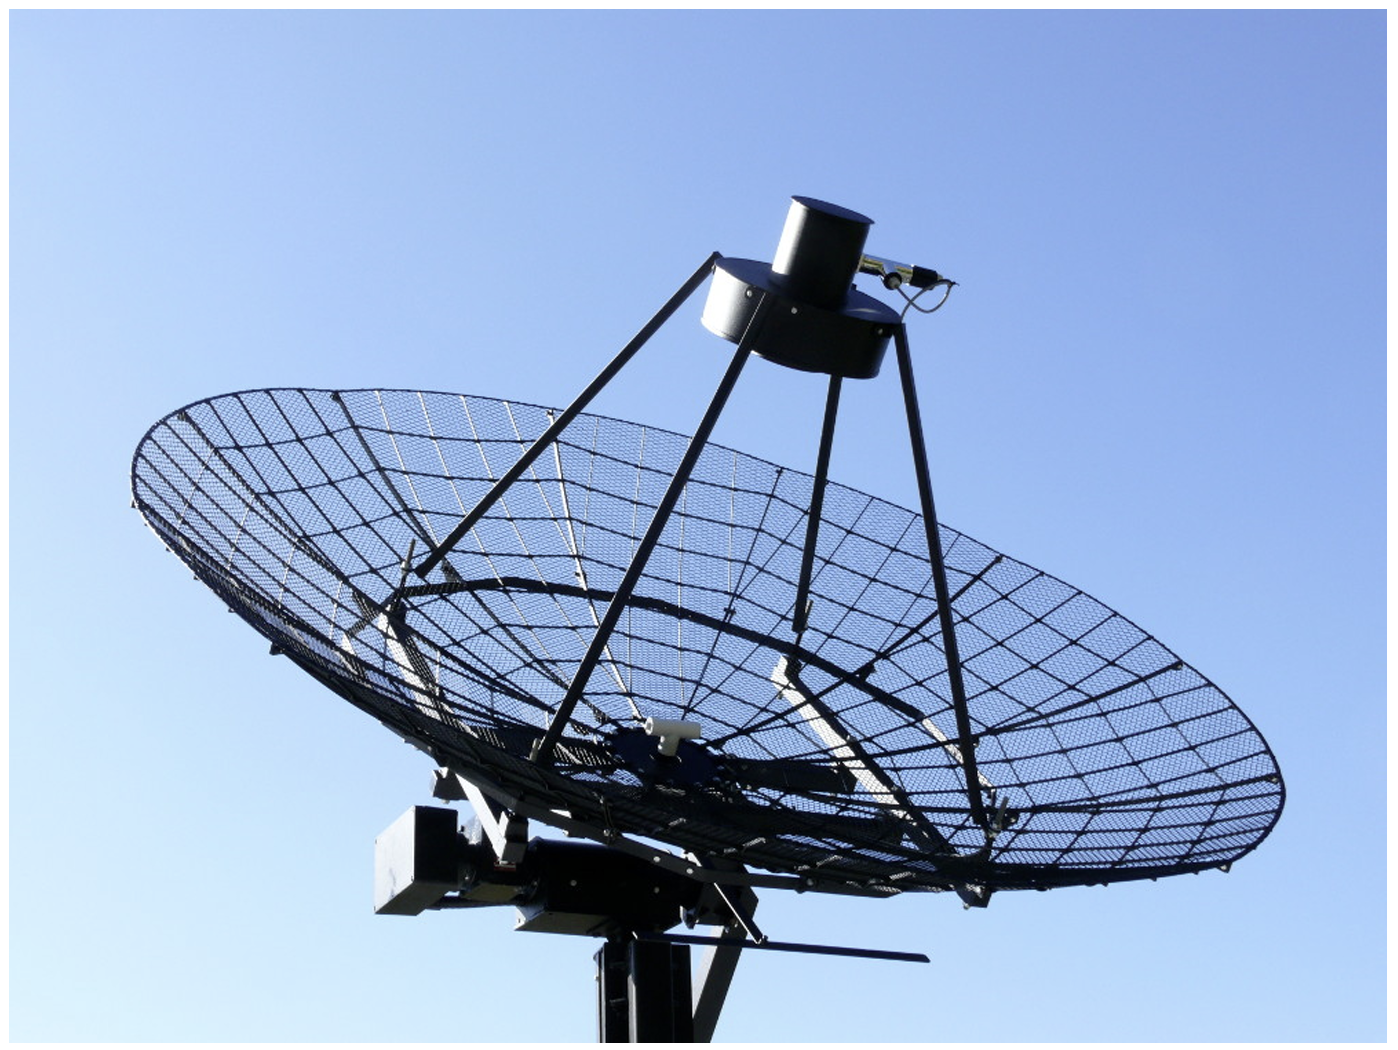
\includegraphics[width=0.5\textwidth]{telescope.png}
            \caption{Radio telescope at Sand 1, Tübingen}
            \label{fig:telescope}
        \end{figure}

        The telescope is on a Alt-Az mount. Using the computer, the telescope can be moved by specifying galactic, equatorial and other coordinate systems.
    \subsection{Observations}
            To start the observations, first a restart of the computer is required. The program qradio is started with the following configurations:\ref{fig:qradio_config}
            \begin{figure}[H]
                \centering
                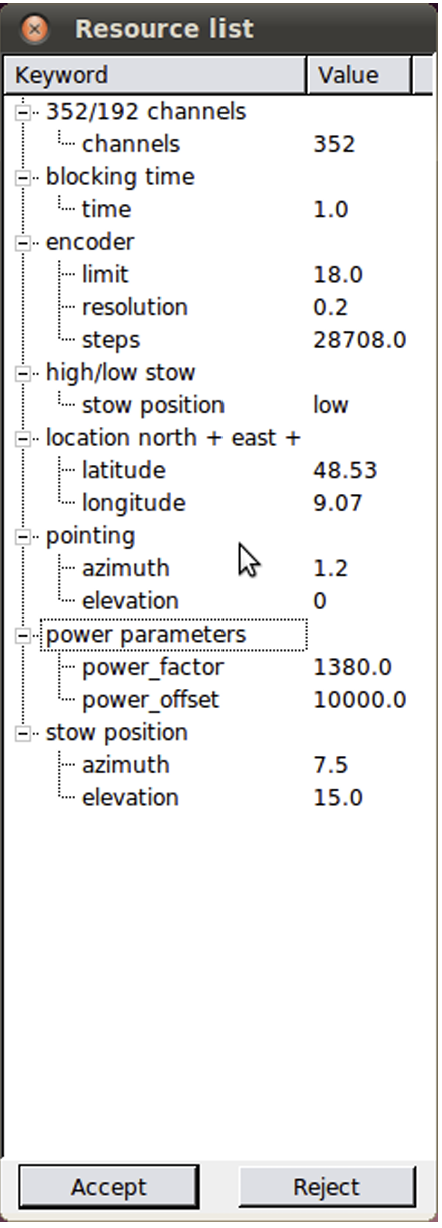
\includegraphics[width=0.15\textwidth]{qradio_config.png}
                \caption{qradio configuration. All the shown values much match}
                \label{fig:qradio_config}
            \end{figure} 

            Now using the GUI, different parameters are set for the observations of the sun and the Milky Way.

            \begin{figure}[H]
                \centering
                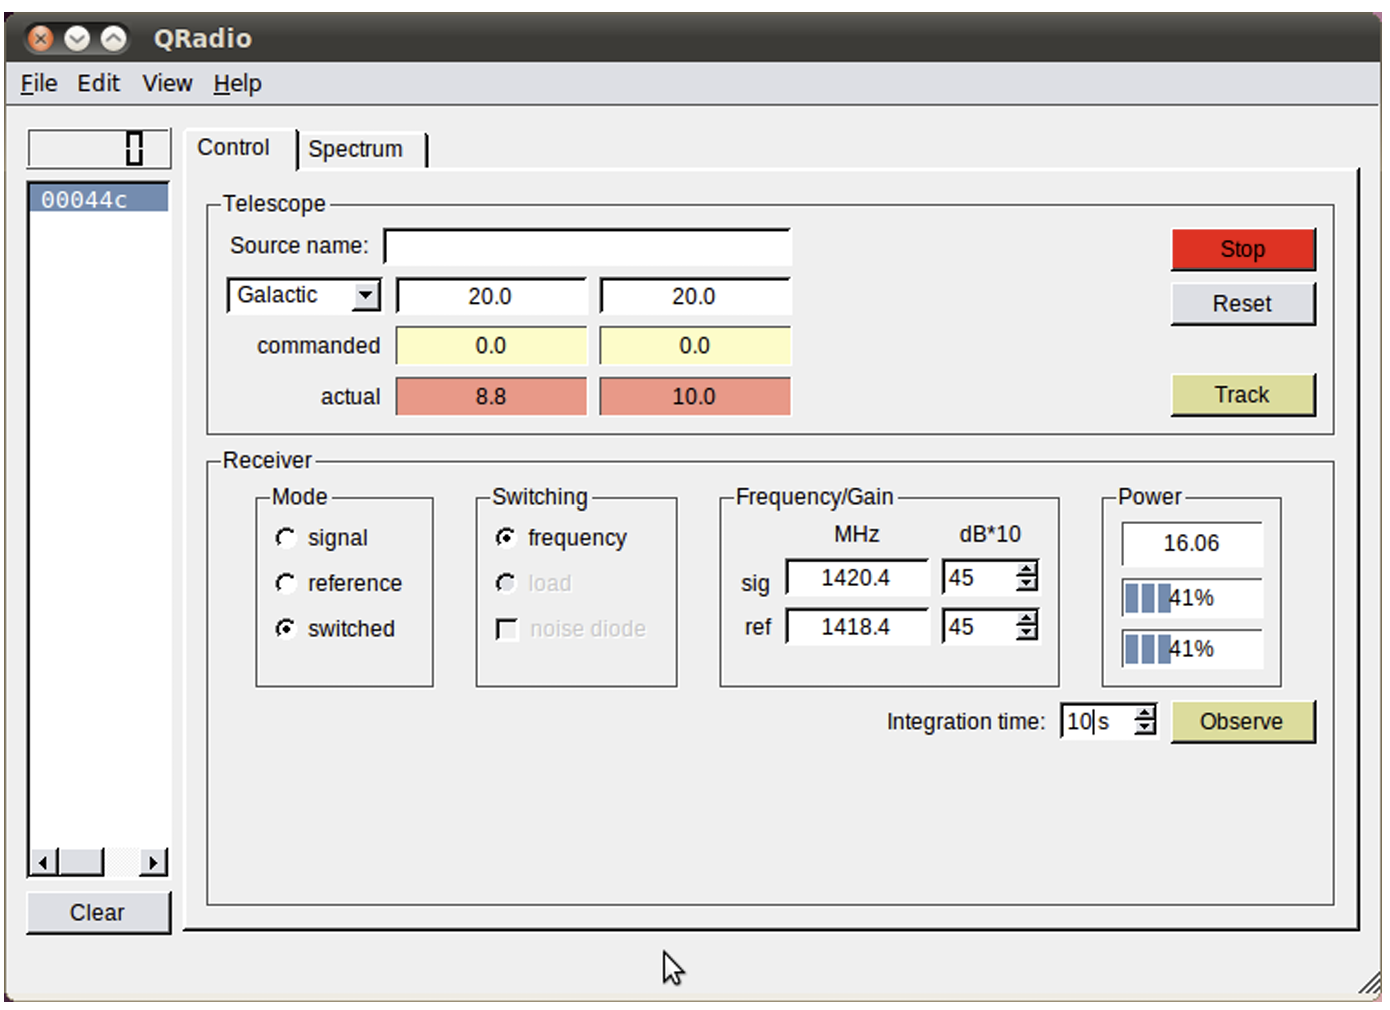
\includegraphics[width=0.5\textwidth]{qradio_gui.png}
                \caption{the qradio GUI}
                \label{fig:qradio_gui}
            \end{figure}
        \subsubsection{Observation of the Sun}
        \subsubsection{Observation of the Milky Way Disk}
            To observe the Milky Way, the following parameters were set:
            \begin{enumerate}
                \item In the \textit{receiver} box, \textit{Mode} is set as `switched' with \textit{Switching} set to `frequency'.
                \item In the \textit{Frequency/Gain} box, $dB*10$ is adjusted such that both signal and reference levels are about $30\%$. We set the it to 30.
                \item We set the coordinates in the \textit{Telescope} box by first setting the coordinate system as `Galactic'. The coordinates are then entered in degrees.
                \item By clicking on \textit{Track} the telescope will move to the required position and will track that coordinate over time.
                \item The spectrum is observed by setting an \textit{integration time} of 10 seconds and by clicking \textit{observe}. The spectrum can then be inspected in the \textit{Control} tab and can be saved.
                \item Next we track and get the spectrum for several sets of coordinates. 
            \end{enumerate}
            
            To choose the coordinates to observe, we first start with part of the disk that is closest to setting in the west anc continue eastward. Spectrums are obtained for $l=25^\circ,30^\circ,40^\circ \dots 80^\circ, 89^\circ$ as b is kept constant at $b=0^\circ$ since we are observing the centre of the disk. \\

            Background measurements are taken at $l=30^\circ,50^\circ,80^\circ$ and $b=30^\circ$ to be subtracted from the previous set of observations.

    \subsection{Data Analysis}

\section{Conclusions}


\printbibliography     
\appendix
\section{Appendix}

\end{document}

